\documentclass[11pt,letterpaper,oneside]{report}
\usepackage[T1]{fontenc}
\usepackage[utf8]{inputenc}
\usepackage[english]{babel}
\usepackage{lmodern}
\usepackage{microtype}
\usepackage[margin=0.86in,headheight=16pt]{geometry}
\usepackage[table,dvipsnames]{xcolor}
\usepackage{graphicx}
\usepackage{booktabs,tabularx,longtable,array}
\usepackage{enumitem}
\usepackage{titlesec}
\usepackage{fancyhdr}
\usepackage{hyperref}
\usepackage{xurl}
\Urlmuskip=0mu plus 1mu\relax
\usepackage{tcolorbox}
\usepackage{listings}
\usepackage{tikz}
\usetikzlibrary{arrows.meta,positioning,shapes.geometric,fit,calc}
\usepackage{needspace}
\usepackage{amssymb}
\definecolor{ink}{HTML}{14253A}
\definecolor{navy}{HTML}{17385D}
\definecolor{blue}{HTML}{20739A}
\definecolor{pale}{HTML}{ECF4F8}
\definecolor{green}{HTML}{1D6C5C}
\definecolor{softgreen}{HTML}{EEF8F4}
\definecolor{border}{HTML}{D4DFE7}
\definecolor{grey}{HTML}{506174}
\hypersetup{colorlinks=true,linkcolor=navy,urlcolor=blue,pdfauthor={Micro-Frontend Engineering Documentation Suite}}
\titleformat{\chapter}[display]{\normalfont\sffamily\bfseries\color{ink}}{\Large\color{blue}\MakeUppercase{\chaptername} \thechapter}{8pt}{\Huge}
\titlespacing*{\chapter}{0pt}{-10pt}{24pt}
\titleformat{\section}{\Large\sffamily\bfseries\color{navy}}{\thesection}{0.7em}{}
\titleformat{\subsection}{\large\sffamily\bfseries\color{navy}}{\thesubsection}{0.6em}{}
\setlist[itemize]{itemsep=3pt,topsep=5pt,leftmargin=1.6em}
\setlist[enumerate]{itemsep=4pt,topsep=5pt,leftmargin=1.8em}
\pagestyle{fancy}\fancyhf{}
\fancyhead[L]{\footnotesize\sffamily MICRO-FRONTEND ENGINEERING SUITE}
\fancyhead[R]{\footnotesize\sffamily\docshort}
\fancyfoot[L]{\footnotesize\color{grey}Engineering edition | October 2026}
\fancyfoot[R]{\footnotesize\thepage}
\renewcommand{\headrulewidth}{0.35pt}
\renewcommand{\arraystretch}{1.2}
\setlength{\emergencystretch}{2em}
\lstdefinestyle{eng}{basicstyle=\ttfamily\footnotesize,keywordstyle=\color{navy}\bfseries,commentstyle=\color{grey},stringstyle=\color{green},breaklines=true,breakatwhitespace=false,columns=fullflexible,keepspaces=true,showstringspaces=false,frame=single,rulecolor=\color{border},backgroundcolor=\color{pale},xleftmargin=5pt,xrightmargin=5pt,aboveskip=10pt,belowskip=10pt,captionpos=b}
\lstdefinelanguage{JavaScript}{morekeywords={const,let,var,require,return,async,await,import,export,default,function,try,catch,new,true,false,undefined,module},sensitive=true,morecomment=[l]//,morestring=[b]',morestring=[b]"}
\lstset{style=eng}
\newtcolorbox{sourcebox}{colback=pale,colframe=border,arc=2pt,boxrule=0.6pt,left=8pt,right=8pt,top=7pt,bottom=7pt}
\newtcolorbox{engineerbox}{colback=softgreen,colframe=green!45,arc=2pt,boxrule=0.6pt,left=8pt,right=8pt,top=7pt,bottom=7pt}
\newcommand{\based}[1]{\begin{sourcebox}\textbf{BOOK-GROUNDED CONCEPT}\\#1\end{sourcebox}}
\newcommand{\added}[1]{\begin{engineerbox}\textbf{ENGINEERING EXTENSION}\\#1\end{engineerbox}}
\newcommand{\term}[1]{\textbf{\color{navy}#1}}
\newcommand{\criterion}[1]{\textbf{Acceptance:} #1}
\newcommand{\book}{\emph{Building Micro-Frontends}, 2nd ed.}
\newcommand{\refs}{\chapter*{References and Provenance}\addcontentsline{toc}{chapter}{References and Provenance}
\begin{enumerate}[leftmargin=*]
\item \textbf{Primary source:} Luca Mezzalira, \emph{Building Micro-Frontends: Distributed Systems for the Frontend}, 2nd ed., O'Reilly Media, published November 2025 (copyright 2026), ISBN 978-1-098-17078-3. Chapter and printed-page references are included throughout. This suite paraphrases and synthesizes concepts; it does not reproduce the book.
\item \textbf{Engineering extension:} Webpack Module Federation reference: \url{https://webpack.js.org/plugins/module-federation-plugin}.
\item \textbf{Engineering extension:} Next.js multi-zones: \url{https://nextjs.org/docs/app/guides/multi-zones}. Details are version-sensitive and must be checked against the deployed framework version.
\item \textbf{Engineering extension:} OWASP Application Security Verification Standard 5.0: \url{https://owasp.org/www-project-application-security-verification-standard/}.
\item \textbf{Engineering extension:} GitHub Actions secure use reference: \url{https://docs.github.com/en/actions/reference/security/secure-use}.
\end{enumerate}}

\titleclass{\chapter}{straight}\titleformat{\chapter}[hang]{\huge\sffamily\bfseries\color{navy}}{\thechapter}{.7em}{}\titlespacing*{\chapter}{0pt}{24pt}{13pt}
\newcommand{\docshort}{DEVSECOPS / CI-CD}
\begin{document}
\begin{titlepage}\thispagestyle{empty}
\vspace*{1.1in}{\Huge\sffamily\bfseries\color{navy} DevSecOps and CI/CD Engineering Guide\par}
\vspace{18pt}{\Large\sffamily\color{blue} Secure software delivery, release discovery, pipeline verification, and production operations\par}
\vspace{27pt}\noindent\color{blue}\rule{0.75\textwidth}{1.4pt}
\vspace{23pt}\par{\large\sffamily A companion to Luca Mezzalira's \emph{Building Micro-Frontends}, Second Edition}\par
\vfill\noindent\textbf{Document series:} Micro-Frontend Software Architecture and Engineering\\
\textbf{Version:} 1.0 \quad \textbf{Prepared:} October 2026\\
\textbf{Production format:} pdfLaTeX-compatible standalone source\\
\textbf{Scope:} Original synthesis plus explicitly identified engineering extensions
\end{titlepage}
\pagenumbering{roman}\tableofcontents\clearpage\pagenumbering{arabic}

\chapter{Security and Delivery Architecture}
\based{Chapters 6--8 cover automation principles, environment/repository strategies, testing, fitness functions, observability, discovery, blue-green/canary releases, and a pipeline case study. Security gates, supply-chain controls, and example workflow below are engineering extensions.}
\section{Security objectives}
Protect the code supply chain, artifact provenance, discovery registry, remote JavaScript origins, session boundaries, backend authorization, and customer data. Build pipelines must fail closed on critical integrity, provenance, or release-contract failures. Browser composition is not a sandbox by default.
\section{Threat model by boundary}
\begin{longtable}{p{.24\linewidth}p{.34\linewidth}p{.32\linewidth}}\toprule Boundary / threat & Abuse scenario & Recommended verification \\\midrule
Source and dependencies & Compromised package executes at build or in browser & Pin/lock dependencies; review changes; SCA, malware checks as applicable\\
CI identity & Untrusted PR obtains write/cloud credentials & Least-privilege permissions, isolated untrusted jobs, OIDC trust scoping\\
Artifact registry & Mutable bytes behind an approved version & Content-addressed artifacts, integrity verification, publish-once semantics\\
Discovery manifest & Attacker retargets a remote URL & Authenticated writes, origin allowlist, audit log, change approval\\
Remote JS & Third-party code executes with origin privileges & Trusted code only, constrained origin policy, layered code review\\
Session/API & UI protection bypassed or data crossed between tenants & Server authorization, secure cookies, CSRF controls where applicable\\
Client telemetry & PII/secret in browser logs & Redaction, sampling, retention and permission controls\\\bottomrule\end{longtable}
\chapter{Pipeline Stages and Release Gates}
\begin{center}\small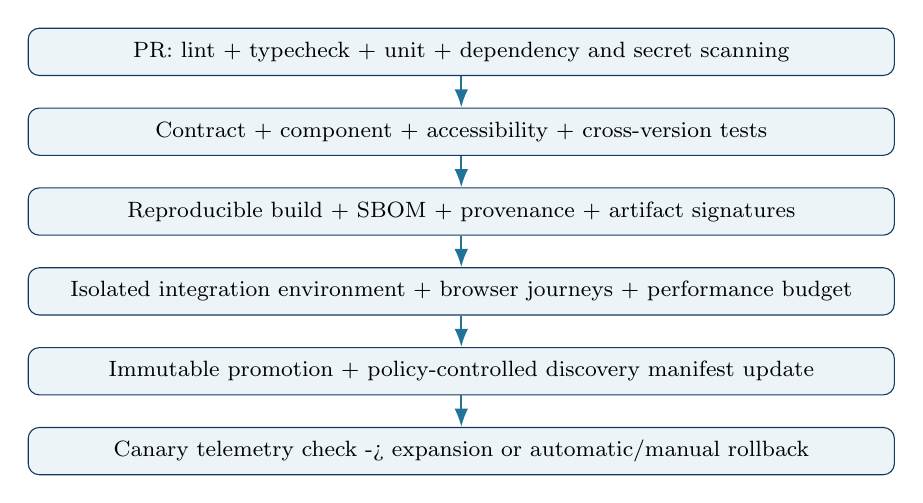
\begin{tikzpicture}[node distance=4mm, every node/.style={font=\footnotesize}, stage/.style={draw=navy,rounded corners,fill=pale,minimum height=.6cm,minimum width=11cm,align=center},arr/.style={-{Latex},draw=blue,thick}]
\node[stage] (a) {PR: lint + typecheck + unit + dependency and secret scanning};
\node[stage,below=of a] (b) {Contract + component + accessibility + cross-version tests};
\node[stage,below=of b] (c) {Reproducible build + SBOM + provenance + artifact signatures};
\node[stage,below=of c] (d) {Isolated integration environment + browser journeys + performance budget};
\node[stage,below=of d] (e) {Immutable promotion + policy-controlled discovery manifest update};
\node[stage,below=of e] (f) {Canary telemetry check -> expansion or automatic/manual rollback};
\foreach \x/\y in {a/b,b/c,c/d,d/e,e/f}{\draw[arr](\x)--(\y);}
\end{tikzpicture}\end{center}
\section{Recommended gate definitions}
\begin{longtable}{p{.2\linewidth}p{.38\linewidth}p{.32\linewidth}}\toprule Gate & Minimum evidence & Failure response \\\midrule
Code quality & Lint, typecheck, unit tests, review & Block merge\\
SAST/CodeQL & Defined repository scanning policy; reviewed actionable findings & Block according to organization risk policy\\
Secret scanning & No untriaged verified credential exposure & Contain and revoke affected keys\\
Dependency/SBOM & Policy-compliant component inventory and risk review & Patch, exception, or reject\\
Contract compatibility & Producer/consumer tests pass against supported versions & Reject promotion\\
Browser integration & Core journeys; auth/forbidden; a11y smoke & Hold release\\
Artifact integrity & Immutable digest tied to commit and build evidence & Reject deploy\\
Canary health & Error rate/latency/business KPI guardrails & Freeze rollout; restore known-good release\\\bottomrule\end{longtable}
\added{Risk thresholds should be organization-approved and business-contextual; raw vulnerability counts, a single CVSS threshold, or success percentages alone are not a substitute for exploitability, exposure, compensating controls, and documented exceptions.}
\chapter{GitHub Actions Implementation Pattern}
\section{Least-privilege PR workflow}
\begin{lstlisting}[caption={Workflow skeleton; replace actions with verified full-length commit SHA references}]
name: domain-ci
on:
  pull_request:
    paths: ['apps/catalog/**', 'packages/domain-contracts/**']
permissions:
  contents: read
jobs:
  validate:
    runs-on: ubuntu-latest
    timeout-minutes: 20
    steps:
      # Replace the action below with a verified full commit SHA.
      - uses: actions/checkout@REPLACE_WITH_VERIFIED_FULL_SHA
        with:
          persist-credentials: false
      # Use a reviewed and SHA-pinned Node setup action.
      - run: npm ci
      - run: npm run lint --workspace=apps/catalog
      - run: npm run typecheck --workspace=apps/catalog
      - run: npm run test --workspace=apps/catalog
      - run: npm run test:contracts --workspace=apps/catalog
\end{lstlisting}
\noindent \textbf{Important:} This intentionally non-runnable template avoids inventing real commit SHAs. Replace placeholders with verified pinned actions, specify approved Node runtime, and apply repository rulesets and required checks. Add CodeQL and dependency scanning using official integrations appropriate to the organization's license and language support. Avoid privileged \texttt{pull\_request\_target} execution of untrusted PR code.
\section{Deployment pipeline separation}
Publish an immutable build artifact once, attest or record provenance, then \emph{promote the same bytes} from test to staging to production. A deployment workflow acquires environment-scoped permissions only after required approvals and checks. Federated credentials should bind allowed repository, branch, workflow, and environment claims when supported.
\chapter{Artifact and Discovery Integrity}
\section{Release manifest record}
\begin{lstlisting}[caption={Illustrative artifact record, not an official schema}]
{
  "domain": "catalog",
  "commit": "<40-char-git-revision>",
  "artifactDigest": "sha256:<validated-artifact-digest>",
  "sbomLocation": "artifact://catalog/sbom.json",
  "contractVersion": "2.1",
  "buildEvidence": "artifact://catalog/provenance.json",
  "deploymentTarget": "staging"
}
\end{lstlisting}
Store artifact digests and approvals in an auditable deployment system. A remote entry file pointing to content-hashed chunks must be promoted consistently with those chunks. Make rollback select the previous immutable release rather than rebuilding from a moving branch.
\section{Feature flags and rollout assignment}
Use discovery/routing for percentage allocations between deployable micro-frontend versions; reserve feature flags for true runtime behavior control. Assign users consistently across a journey (sticky cohort assignment) to avoid mixing incompatible checkout steps. Do not use client-controlled cohort cookies as a security or pricing decision.
\chapter{Testing Strategy and Fitness Functions}
\section{Layered suite}
\begin{enumerate}\item Unit tests: pure rendering, business validation, accessibility primitives.
\item Contract tests: module exports, events, route ownership, API schemas.
\item Integration tests: shell loading, remote lifecycle, shared dependencies, BFF responses.
\item Browser E2E: purchase journey, identity continuity, deep-link and back-button behavior.
\item Failure tests: DNS/CDN outage, stale manifest, missing chunk, API timeout, conflicting remote versions.
\item Nonfunctional tests: bundle budgets, keyboard/focus, core web vitals and security headers.\end{enumerate}
\section{Fitness function examples}
\begin{tabularx}{\linewidth}{p{.35\linewidth}X}\toprule Function & Example assertable condition \\\midrule
Domain dependency cycles & Build fails on any prohibited cyclic import between domains\\
Route ownership & Every production route maps to exactly one accountable domain\\
Trusted remote source & Every manifest URL matches an approved origin and deployment record\\
Backward compatibility & Current shell loads present and prior supported remotes in tests\\
Accessibility smoke & No critical automated violations, plus manual keyboard acceptance\\
Performance budget & Domain route meets explicitly set JS and interaction budgets\\\bottomrule\end{tabularx}
\chapter{Operations, SLOs, and Recovery}
\section{Telemetry contract}
Every domain release emits build/release ID and route; correlation connects the browser, edge, BFF, and service spans. Measure remote load failures, browser errors by version, API latency, origin/cache status, checkout drop-off, and deployment cohorts. Never attach tokens or personal data to metrics attributes.
\section{Suggested SLO definition}
Define each SLI before setting a target: e.g., \emph{successful checkout initiation requests / eligible checkout initiation attempts} by production route, with explicit exclusions. Track error-budget burn, not only overall page availability. Establish release rollback thresholds from observed baselines and risk appetite, not an invented universal percentage.
\section{Incident runbook}
\begin{enumerate}\item Identify affected domain, release, cohort, route, and time of onset.
\item Disable further promotion; freeze manifest mutation if tampering is suspected.
\item Repoint discovery to known-good artifact or reroute a zone.
\item Confirm cache invalidation and consistency across regions.
\item Verify the core user journey, identity, error rates, and performance recovery.
\item Preserve evidence; write incident review and update architecture fitness functions.\end{enumerate}
\chapter{Security Control Acceptance Matrix}
\begin{longtable}{p{.2\linewidth}p{.3\linewidth}p{.38\linewidth}}\toprule Control ID & Control statement & Evidence \\\midrule
MF-SEC-01 & Sensitive operations authorize at backend & Denied access integration tests\\
MF-SEC-02 & Remote entry origins are approved & Policy tests and manifest review\\
MF-SEC-03 & Build has reviewed source/dependency provenance & SBOM, digest, build record\\
MF-SEC-04 & CI secrets inaccessible to untrusted code & Permissions inspection and PR test\\
MF-SEC-05 & Session consistency across zones & Logout, expiry, CSRF tests\\
MF-SEC-06 & Client and server logs avoid secrets and PII & Synthetic leakage tests, telemetry schema\\
MF-SEC-07 & Rollback is exercised and time-bounded & Signed-off drill record and deployment history\\
MF-SEC-08 & Security exceptions expire and are owned & Risk acceptance entry and review date\\\bottomrule\end{longtable}

\refs
\end{document}
